\documentclass[11pt,letter,DIV=14,paper=landscape]{scrbook}
\usepackage{typearea}
\pagestyle{plain}
\setcounter{secnumdepth}{1}
\usepackage{etoolbox}
\usepackage{graphicx}
\usepackage{fancyvrb}
\usepackage[T1]{fontenc}
\usepackage{url}
\usepackage[hidelinks=true,linktoc=all]{hyperref}
\urlstyle{same}
\setlength{\parindent}{0em}
\setlength{\parskip}{1ex}
\usepackage{verbatim}
\usepackage{listings}
\usepackage{caption}
\graphicspath{{/Users/michaelgogins/Dropbox/images/}{/Users/michaelgogins/Dropbox/images/renamed}{/Users/michaelgogins/Dropbox/images/XT_1585/Camera}{/Users/michaelgogins/Dropbox/images/duplicates}{/Users/michaelgogins/Dropbox/images/SM-950U}{/Users/michaelgogins/Dropbox/images/RX100M5/100MSDCF}{/Users/michaelgogins/Dropbox/images/RX100/100MSDCF}}
\DeclareTOCStyleEntry[numwidth=3em]{tocline}{figure}
\begin{document}
\frontmatter

\title{A Third Eye Made of Glass}
\subtitle{Volume I }
\author{Michael Gogins \\ \texttt{michael.gogins@gmail.com}}
\date{2022 }
\publishers{Irreducible Productions, New York}

\maketitle
	
\clearpage
\thispagestyle{empty}
\noindent This book and all images herein are copyright 2020 by Michael Gogins, all rights reserved. This book and its contents are licensed under the terms of the Creative Commons \href{https://creativecommons.org/licenses/by-nc-nd/4.0/legalcode}{\textbf{Attribution-NonCommercial-NoDerivatives 4.0 International} } license. 

In short, you may use, print, and copy this book or any of its contents for your own personal use, but you may not use this book or any of its contents as part of your own projects, or for commercial purposes.

If you wish to use this book or any of its contents for your own projects, or for commercial purposes, for example to re-publish or to exhibit in a gallery, please contact me directly.

This book was typeset by me using LaTeX2e and the KOMA-Script bundle. I wrote Python code to extract metadata from photographs, print descriptions of them, and format everything as proper LaTeX.

\clearpage
\thispagestyle{empty}
\begin{center}
\vspace*{\stretch{1}}
\emph{This book is for Mick.}
\vspace*{\stretch{3}}
\end{center}

\clearpage
\tableofcontents

\mainmatter
\lstset{language=c++,basicstyle=\ttfamily\scriptsize,commentstyle=\ttfamily\tiny,tabsize=2,breaklines,fontadjust=true,keepspaces=false,showstringspaces=false,moredelim=[is][\textbf]{\\emph\{}{\}}}

\setlength{\columnsep}{3em}
\twocolumn

\chapter{Introduction}

This book contains my selection of pictures from a lifetime of taking photographs. I have never been a professional, but I was and am committed to the art of photography. I am a ``street photographer'' open to abstraction. I shoot what catches my eye, and I prize beauty. When I take pictures of people, I usually prefer they don't notice. My reason for doing photography is to see more clearly what God has created.

These pictures were variously taken with 35 mm film cameras, a variety of digital cameras, and smartphones. They were taken in my native state of Utah, other states including Washington, California, and New York, and countries around the world. I have tended to use the sharpest possible camera that is small enough to carry with me at all times. For some years now I have been using the Sony RX100 series. Increasingly, however, I am finding that my smartphone is a real camera.

The images are all in natural color. They are all shot as far as possible without image manipulation; in a few cases, I have leveled horizons or removed spots. I shoot in JPEG rather than RAW. Selected metadata from the photographs is printed. If the photograph is a digital scan of a 35 mm slide, the creation date is the date of that scan. Captions are incomplete and cryptic. Images are, to the best of my recollection where timestamps are lacking, in chronological order.

\emph{All pictures are included in the full resolution with which they were taken}. Thus, you can zoom into any image to see more detail. Pictures copied out of this book will also be in full resolution. As the file size of this book would otherwise become unmanageable thanks to the use of uncompressed images, it has been split into volumes of no more than about 500 megabytes each. Even so, the files are huge.

I invite the reader to copy pictures out of this book for printing and viewing, but not for commercial use or re-publication. 

\begin{table}[h]
\centering
\captionsetup{labelformat=empty}
\caption{\textbf{Maximum Recommended Print Sizes}}
\begin{tabular}{lrr}
\hline
Source                       & Close up & On the wall  \\
\hline
35 mm Velvia slide (for comparison) & 16" x 20" & 18" x 24" \\
My scans of slides                            & 11" x 14"  & 16" x 20"  \\
20 megapixel digital camera             & 16" x 20"  & 18" x 24"  \\
High-end smartphone                      & 8" x 10"   & Up to 16" x 20"  \\
\hline
\end{tabular}
\end{table}

If I take more pictures that I think are good enough to be in this book, I will add new volumes.
	
	
\onecolumn
\chapter{Photographs}
\clearpage



\clearpage
\emph{This book is for Mick.}
\clearpage

\tableofcontents

\mainmatter
\lstset{language=c++,basicstyle=\ttfamily\scriptsize,commentstyle=\ttfamily\tiny,tabsize=2,breaklines,fontadjust=true,keepspaces=false,showstringspaces=false,moredelim=[is][\textbf]{\\emph\{}{\}}}

%\pagestyle{headings}
\setlength{\columnsep}{3em}
\twocolumn

\chapter{Introduction}

This book contains my selection of pictures from a lifetime of taking photographs. I have never been a professional, but I was and am committed to the art of photography. I am a ``street photographer'' open to abstraction. I shoot what catches my eye, and I prize beauty. When I take pictures of people, I usually prefer they don't notice. My reason for doing photography is to see more clearly what God has created.

These pictures were variously taken with 35 mm film cameras, a variety of digital cameras, and smartphones. They were taken in my native state of Utah, other states including Washington, California, and New York, and countries around the world. I have tended to use the sharpest possible camera that is small enough to carry with me at all times. For some years now I have been using the Sony RX100 series. Increasingly, however, I am finding that my smartphone is a real camera.

The images are all in natural color. They are all shot as far as possible without image manipulation; in a few cases, I have leveled horizons or removed spots. I shoot in JPEG rather than RAW. Selected metadata from the photographs is printed. If the photograph is a digital scan of a 35 mm slide, the creation date is the date of that scan. Captions are incomplete and cryptic. Images are, to the best of my recollection where timestamps are lacking, in chronological order.

\emph{All pictures are included in the full resolution with which they were taken}. Thus, you can zoom into any image to see more detail. Pictures copied out of this book will also be in full resolution. As the file size of this book would otherwise become unmanageable thanks to the use of uncompressed images, it has been split into volumes of no more than about 500 megabytes each. Even so, the files are huge.

I invite the reader to copy pictures out of this book for printing and viewing, but not for commercial use or re-publication. 

\begin{table}[h]
\centering
\captionsetup{labelformat=empty}
\caption{\textbf{Maximum Recommended Print Sizes}}
\begin{tabular}{lrr}
\hline
Source                       & Close up & On the wall  \\
\hline
35 mm Velvia slide (for comparison) & 16" x 20" & 18" x 24" \\
My scans of slides                            & 11" x 14"  & 16" x 20"  \\
20 megapixel digital camera             & 16" x 20"  & 18" x 24"  \\
High-end smartphone                      & 8" x 10"   & Up to 16" x 20"  \\
\hline
\end{tabular}
\end{table}

If I take more pictures that I think are good enough to be in this book, I will add new volumes.
	
	
\onecolumn
\chapter{Photographs}
\clearpage

% Supposed to generate all contents from the manifest, currently must be done separately
%%immediate\write18{python3 photos-to-latex.py}


%% photos_gathered: 1
\clearpage
\section{\protect\detokenize{c-2013-03-12_12-07-24.jpg}}
\noindent When I was 18 years old, my father Laird gave me a Mamiya Sekor 35mm SLR camera for Christmas. I took this picture in the back yard of Laird's girlfriend Doreen's house in Taylorsville, Utah, just after sunset. I believe this was actually on Christmas Day.
\noindent
\begin{lstlisting}

\end{lstlisting}
\clearpage
\begin{figure}
\raggedleft
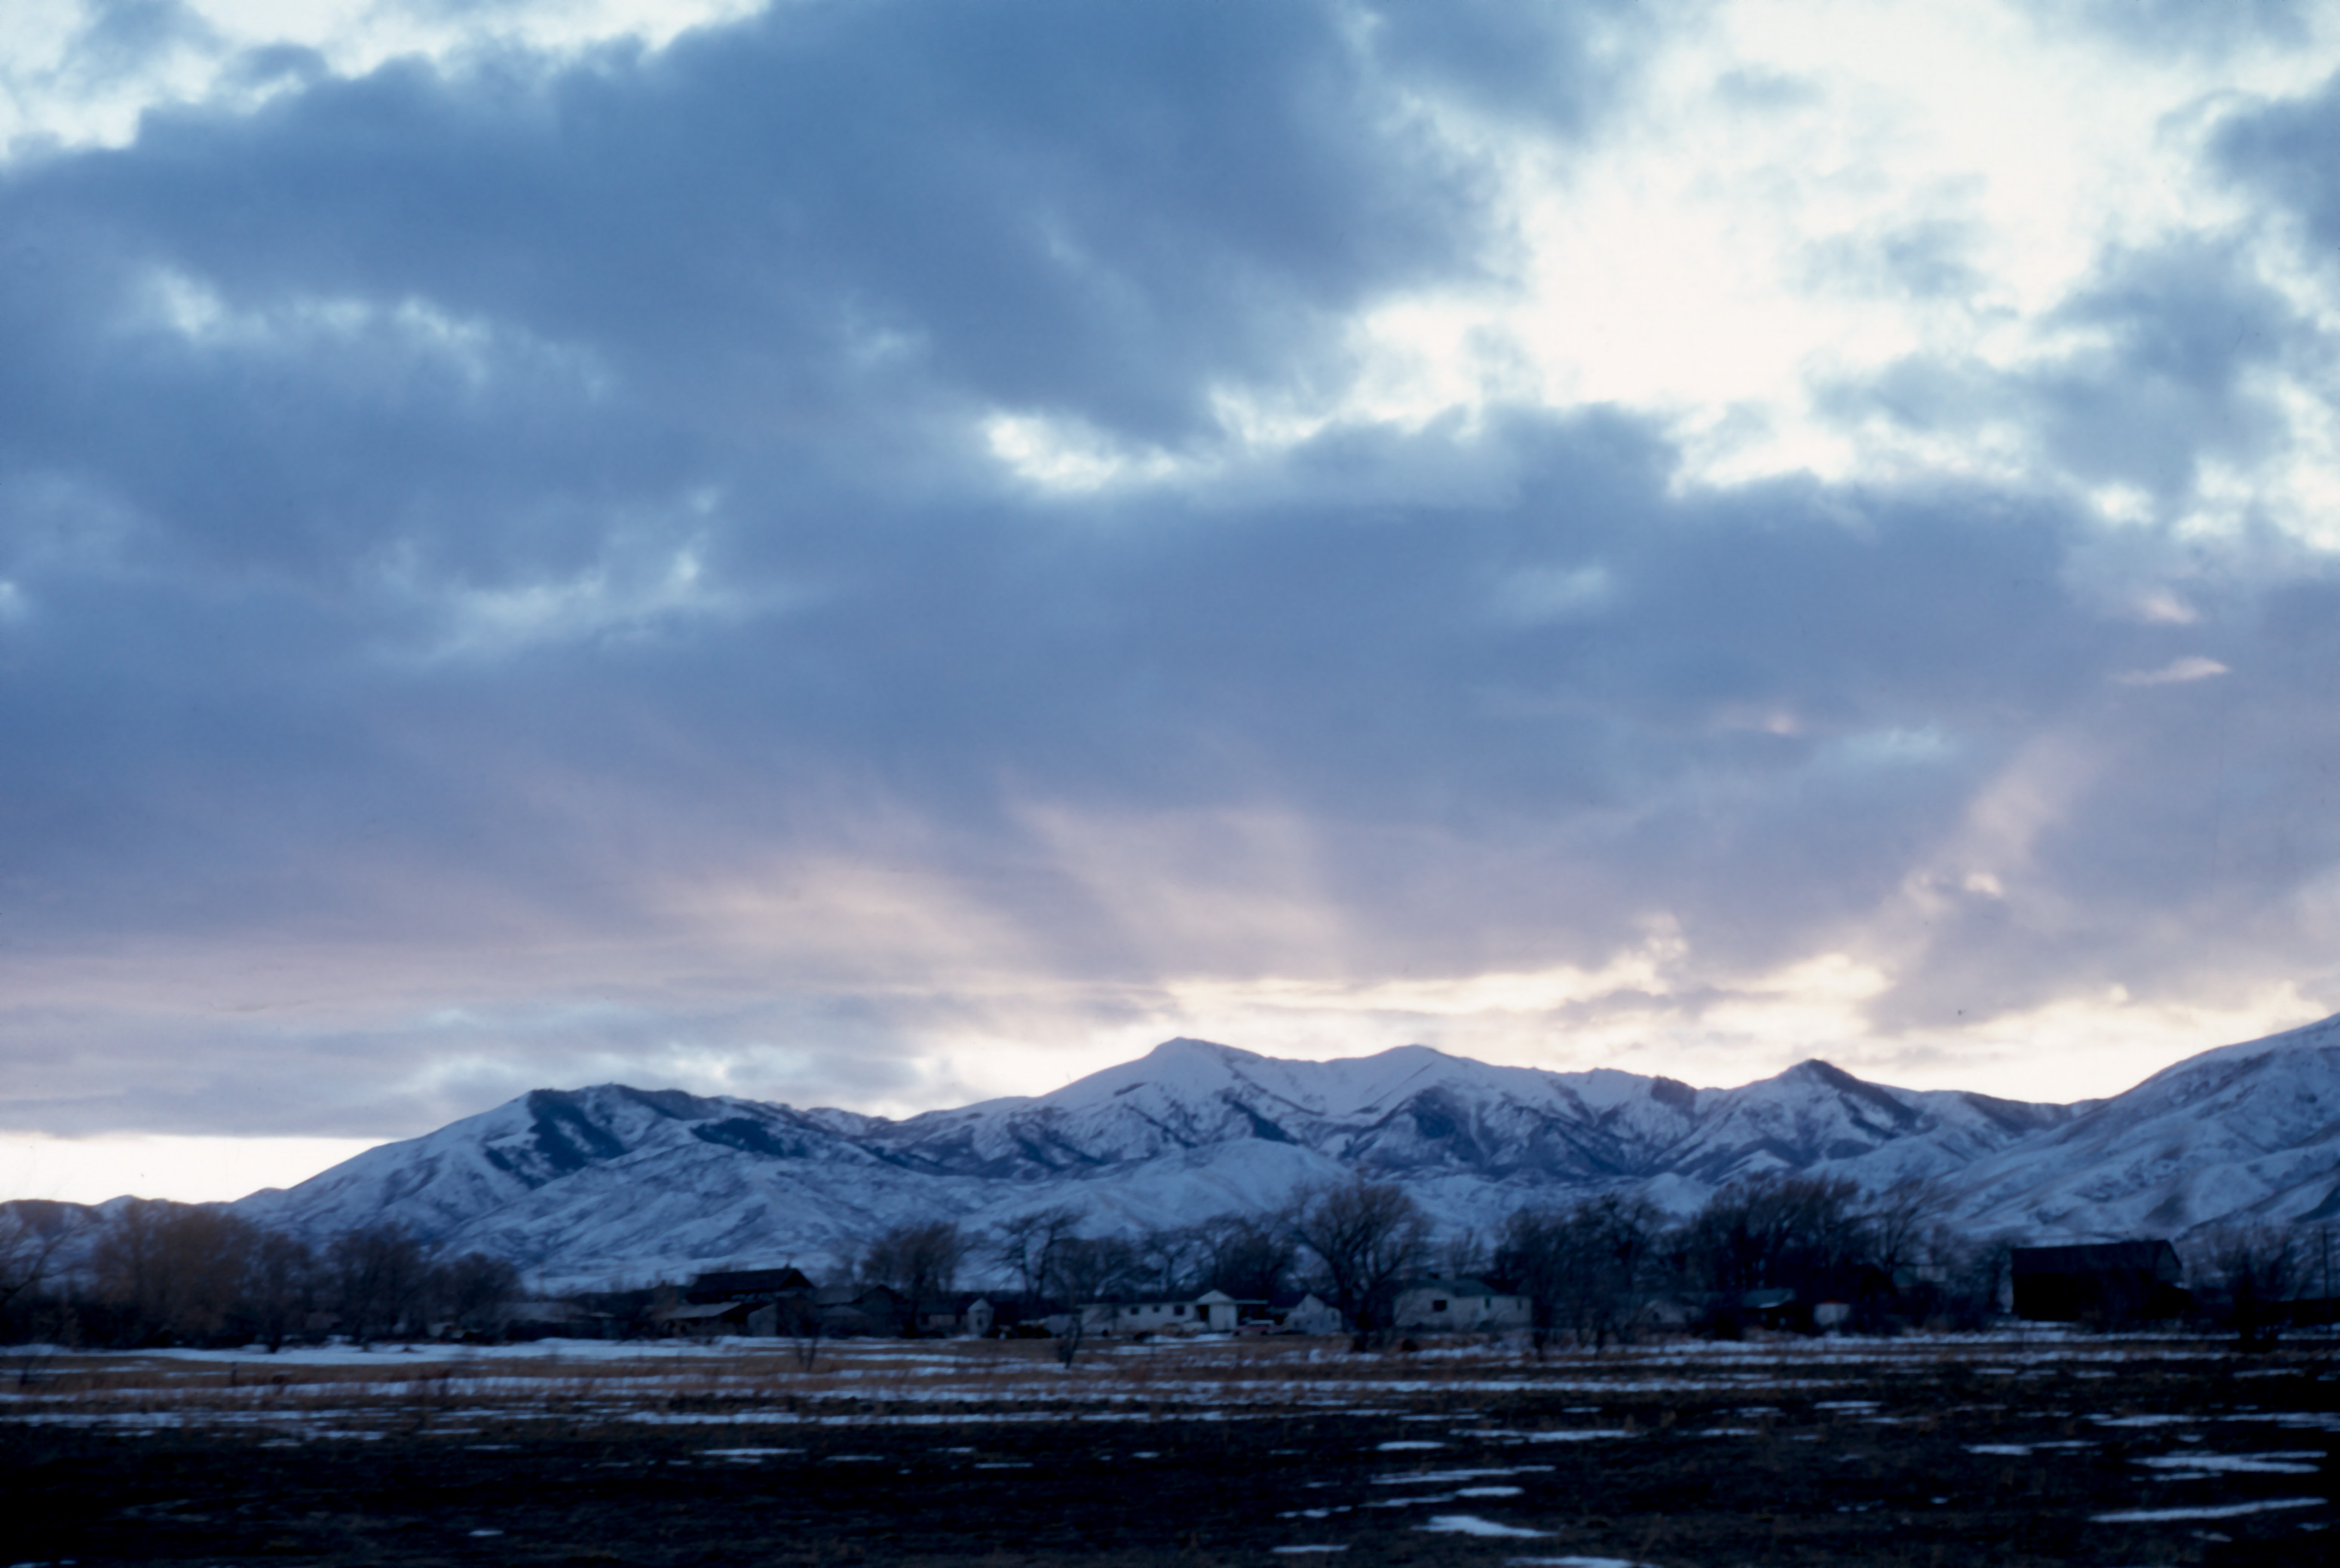
\includegraphics[height=\textheight,width=\linewidth,keepaspectratio]{c-2013-03-12_12-07-24.jpg}
\end{figure}


%% photos_gathered: 2
\clearpage
\section{\protect\detokenize{Mick_Wendy_Jane_Michael_XMas.jpg}}
\noindent Scan of a slide of my grandfather Milton (Mick) Swensen, my sister Wendy, my grandmother Jane, and myself, Murray, Utah, Christmas or New Years 1968 I think.
\noindent
\begin{lstlisting}
Image width:                   2904
Image height:                  1848

\end{lstlisting}
\clearpage
\begin{figure}
\raggedleft
\includegraphics[height=\textheight,width=\linewidth,keepaspectratio]{Mick_Wendy_Jane_Michael_XMas.jpg}
\end{figure}


%% photos_gathered: 3
\clearpage
\section{\protect\detokenize{c_2013-03-11_04-41-39.1.jpg}}
\noindent Scan of a slide of Elaine Constable, to whom I was briefly married, First Avenue stairs, Salt Lake City, Utah, 1971.
\noindent
\begin{lstlisting}
EXIF tag:   271   Make:                          Nikon
EXIF tag:   272   Model:                         Nikon SUPER COOLSCAN 5000 ED
EXIF tag:   305   Software:                      Nikon Scan 4.0.0 W
EXIF tag:   274   Orientation:                   1
EXIF tag:   306   DateTime:                      2006.03.26 16.25.26
EXIF tag: 40962   ExifImageWidth:                5782
EXIF tag: 40963   ExifImageHeight:               3946

\end{lstlisting}
\clearpage
\begin{figure}
\raggedleft
\includegraphics[height=\textheight,width=\linewidth,keepaspectratio]{c_2013-03-11_04-41-39.1.jpg}
\end{figure}


%% photos_gathered: 4
\clearpage
\section{\protect\detokenize{c_2013-03-11_04-41-41.1.jpg}}
\noindent Scan of a slide, sidewalk leaves, South Temple Street, Salt Lake City, Utah, 1972.
\noindent
\begin{lstlisting}
EXIF tag:   271   Make:                          Nikon
EXIF tag:   272   Model:                         Nikon SUPER COOLSCAN 5000 ED
EXIF tag:   305   Software:                      Nikon Scan 4.0.0 W
EXIF tag:   274   Orientation:                   1
EXIF tag:   306   DateTime:                      2006.03.26 16.35.14
EXIF tag: 40962   ExifImageWidth:                5782
EXIF tag: 40963   ExifImageHeight:               3946

\end{lstlisting}
\clearpage
\begin{figure}
\raggedleft
\includegraphics[height=\textheight,width=\linewidth,keepaspectratio]{c_2013-03-11_04-41-41.1.jpg}
\end{figure}


%% photos_gathered: 5
\clearpage
\section{\protect\detokenize{c_2013-03-11_04-41-44.1.jpg}}
\noindent Scan of a slide, Capitol Hill, Salt Lake City, Utah, 1972.
\noindent
\begin{lstlisting}
EXIF tag:   271   Make:                          Nikon
EXIF tag:   272   Model:                         Nikon SUPER COOLSCAN 5000 ED
EXIF tag:   305   Software:                      Nikon Scan 4.0.0 W
EXIF tag:   274   Orientation:                   1
EXIF tag:   306   DateTime:                      2006.03.26 15.39.32
EXIF tag: 40962   ExifImageWidth:                5782
EXIF tag: 40963   ExifImageHeight:               3946

\end{lstlisting}
\clearpage
\begin{figure}
\raggedleft
\includegraphics[height=\textheight,width=\linewidth,keepaspectratio]{c_2013-03-11_04-41-44.1.jpg}
\end{figure}


%% photos_gathered: 6
\clearpage
\section{\protect\detokenize{c_2013-03-11_04-41-51.1.jpg}}
\noindent Scan of a slide, dry cleaners around the corner from where I lived after separating from Elaine, Salt Lake City, Utah, 1972.
\noindent
\begin{lstlisting}
EXIF tag:   271   Make:                          Nikon
EXIF tag:   272   Model:                         Nikon SUPER COOLSCAN 5000 ED
EXIF tag:   305   Software:                      Nikon Scan 4.0.0 W
EXIF tag:   274   Orientation:                   1
EXIF tag:   306   DateTime:                      2006.03.26 15.54.39
EXIF tag: 40962   ExifImageWidth:                5782
EXIF tag: 40963   ExifImageHeight:               3946

\end{lstlisting}
\clearpage
\begin{figure}
\raggedleft
\includegraphics[height=\textheight,width=\linewidth,keepaspectratio]{c_2013-03-11_04-41-51.1.jpg}
\end{figure}


%% photos_gathered: 7
\clearpage
\section{\protect\detokenize{c_2016-04-06_21-05-56.1_v1.jpg}}
\noindent Scan of a slide of the Deep Creek Mountains, western Utah, 1972 or so.
\noindent
\begin{lstlisting}
EXIF tag:   256   ImageWidth:                    3136
EXIF tag:   257   ImageLength:                   2072
EXIF tag:   305   Software:                      digiKam-5.6.0
EXIF tag: 40962   ExifImageWidth:                3136
EXIF tag: 40963   ExifImageHeight:               2072

\end{lstlisting}
\clearpage
\begin{figure}
\raggedleft
\includegraphics[height=\textheight,width=\linewidth,keepaspectratio]{c_2016-04-06_21-05-56.1_v1.jpg}
\end{figure}


%% photos_gathered: 8
\clearpage
\section{\protect\detokenize{c_2013-03-11_04-42-07.1.jpg}}
\noindent Scan of a slide, Riverside Park, New York City, 1972.
\noindent
\begin{lstlisting}
EXIF tag:   271   Make:                          Nikon
EXIF tag:   272   Model:                         Nikon SUPER COOLSCAN 5000 ED
EXIF tag:   305   Software:                      Nikon Scan 4.0.0 W
EXIF tag:   274   Orientation:                   1
EXIF tag:   306   DateTime:                      2006.03.26 17.30.45
EXIF tag: 40962   ExifImageWidth:                5782
EXIF tag: 40963   ExifImageHeight:               3946

\end{lstlisting}
\clearpage
\begin{figure}
\raggedleft
\includegraphics[height=\textheight,width=\linewidth,keepaspectratio]{c_2013-03-11_04-42-07.1.jpg}
\end{figure}


%% photos_gathered: 9
\clearpage
\section{\protect\detokenize{c_2013-03-11_04-26-22.1.jpg}}
\noindent Scan of a slide taken while hitchiking across the country, 1972 I think.
\noindent
\begin{lstlisting}

\end{lstlisting}
\clearpage
\begin{figure}
\raggedleft
\includegraphics[height=\textheight,width=\linewidth,keepaspectratio]{c_2013-03-11_04-26-22.1.jpg}
\end{figure}


%% photos_gathered: 10
\clearpage
\section{\protect\detokenize{c_2013-03-11_04-41-49.1.jpg}}
\noindent Scan of a slide, coin laundromat, Third Avenue, Salt Lake City, Utah, 1972 or so.
\noindent
\begin{lstlisting}
EXIF tag:   271   Make:                          Nikon
EXIF tag:   272   Model:                         Nikon SUPER COOLSCAN 5000 ED
EXIF tag:   305   Software:                      Nikon Scan 4.0.0 W
EXIF tag:   274   Orientation:                   1
EXIF tag:   306   DateTime:                      2006.03.26 15.50.27
EXIF tag: 40962   ExifImageWidth:                5782
EXIF tag: 40963   ExifImageHeight:               3946

\end{lstlisting}
\clearpage
\begin{figure}
\raggedleft
\includegraphics[height=\textheight,width=\linewidth,keepaspectratio]{c_2013-03-11_04-41-49.1.jpg}
\end{figure}


%% photos_gathered: 11
\clearpage
\section{\protect\detokenize{c_2013-03-11_04-26-23.1.jpg}}
\noindent Scan of a slide taken by a friend with my camera of myself on flute, free jazz jam in Loring Park, Minneapolis, Minnesota, 1973.
\noindent
\begin{lstlisting}
EXIF tag:   271   Make:                          Nikon
EXIF tag:   272   Model:                         Nikon SUPER COOLSCAN 5000 ED
EXIF tag:   305   Software:                      Nikon Scan 4.0.0 W
EXIF tag:   274   Orientation:                   1
EXIF tag:   306   DateTime:                      2006.03.26 16.00.18
EXIF tag: 40962   ExifImageWidth:                5782
EXIF tag: 40963   ExifImageHeight:               3946

\end{lstlisting}
\clearpage
\begin{figure}
\raggedleft
\includegraphics[height=\textheight,width=\linewidth,keepaspectratio]{c_2013-03-11_04-26-23.1.jpg}
\end{figure}


%% photos_gathered: 12
\clearpage
\section{\protect\detokenize{c_2013-03-11_04-41-56.1.jpg}}
\noindent Scan of a slide of my sister Wendy, outside our building in the Loring Park neighborhood, Minneapolis, Minnesota, 1973.
\noindent
\begin{lstlisting}
EXIF tag:   271   Make:                          Nikon
EXIF tag:   272   Model:                         Nikon SUPER COOLSCAN 5000 ED
EXIF tag:   305   Software:                      Nikon Scan 4.0.0 W
EXIF tag:   274   Orientation:                   1
EXIF tag:   306   DateTime:                      2006.03.26 16.59.40
EXIF tag: 40962   ExifImageWidth:                5782
EXIF tag: 40963   ExifImageHeight:               3946

\end{lstlisting}
\clearpage
\begin{figure}
\raggedleft
\includegraphics[height=\textheight,width=\linewidth,keepaspectratio]{c_2013-03-11_04-41-56.1.jpg}
\end{figure}


%% photos_gathered: 13
\clearpage
\section{\protect\detokenize{c_2013-03-11_04-41-52.1.jpg}}
\noindent Scan of a slide, bike on porch, Lake Harriet neighborhood, Minneapolis, Minnesota, 1973.
\noindent
\begin{lstlisting}
EXIF tag:   271   Make:                          Nikon
EXIF tag:   272   Model:                         Nikon SUPER COOLSCAN 5000 ED
EXIF tag:   305   Software:                      Nikon Scan 4.0.0 W
EXIF tag:   306   DateTime:                      2006.03.26 15.56.29
EXIF tag: 40962   ExifImageWidth:                5782
EXIF tag: 40963   ExifImageHeight:               3946

\end{lstlisting}
\clearpage
\begin{figure}
\raggedleft
\includegraphics[height=\textheight,width=\linewidth,keepaspectratio]{c_2013-03-11_04-41-52.1.jpg}
\end{figure}


%% photos_gathered: 14
\clearpage
\section{\protect\detokenize{c_2013-03-11_04-41-57.1.jpg}}
\noindent Scan of a slide, my girlfriend Penny Suess, downtown Minneapolis, Minnesota, 1973.
\noindent
\begin{lstlisting}
EXIF tag:   271   Make:                          Nikon
EXIF tag:   272   Model:                         Nikon SUPER COOLSCAN 5000 ED
EXIF tag:   305   Software:                      Nikon Scan 4.0.0 W
EXIF tag:   274   Orientation:                   1
EXIF tag:   306   DateTime:                      2006.03.26 17.00.59
EXIF tag: 40962   ExifImageWidth:                5782
EXIF tag: 40963   ExifImageHeight:               3946

\end{lstlisting}
\clearpage
\begin{figure}
\raggedleft
\includegraphics[height=\textheight,width=\linewidth,keepaspectratio]{c_2013-03-11_04-41-57.1.jpg}
\end{figure}


%% photos_gathered: 15
\clearpage
\section{\protect\detokenize{c_2013-03-11_04-41-36.1.jpg}}
\noindent Scan of a slide taken at the Minnesota State Fair, 1973.
\noindent
\begin{lstlisting}
EXIF tag:   271   Make:                          Nikon
EXIF tag:   272   Model:                         Nikon SUPER COOLSCAN 5000 ED
EXIF tag:   305   Software:                      Nikon Scan 4.0.0 W
EXIF tag:   306   DateTime:                      2006.03.26 17.46.46
EXIF tag: 40962   ExifImageWidth:                3946
EXIF tag: 40963   ExifImageHeight:               5782

\end{lstlisting}
\clearpage
\begin{figure}
\raggedleft
\includegraphics[height=\textheight,width=\linewidth,keepaspectratio]{c_2013-03-11_04-41-36.1.jpg}
\end{figure}


%% photos_gathered: 16
\clearpage
\section{\protect\detokenize{c_2013-03-11_04-42-06.1.jpg}}
\noindent Scan of a slide, Ferris wheel, Minnesota State Fair, 1973.
\noindent
\begin{lstlisting}
EXIF tag:   271   Make:                          Nikon
EXIF tag:   272   Model:                         Nikon SUPER COOLSCAN 5000 ED
EXIF tag:   305   Software:                      Nikon Scan 4.0.0 W
EXIF tag:   274   Orientation:                   1
EXIF tag:   306   DateTime:                      2006.03.26 17.29.08
EXIF tag: 40962   ExifImageWidth:                5782
EXIF tag: 40963   ExifImageHeight:               3946

\end{lstlisting}
\clearpage
\begin{figure}
\raggedleft
\includegraphics[height=\textheight,width=\linewidth,keepaspectratio]{c_2013-03-11_04-42-06.1.jpg}
\end{figure}


%% photos_gathered: 17
\clearpage
\section{\protect\detokenize{c_2013-03-11_04-42-05.1.jpg}}
\noindent Scan of a slide, ride, Minnesota State Fair, 1973.
\noindent
\begin{lstlisting}
EXIF tag:   271   Make:                          Nikon
EXIF tag:   272   Model:                         Nikon SUPER COOLSCAN 5000 ED
EXIF tag:   305   Software:                      Nikon Scan 4.0.0 W
EXIF tag:   306   DateTime:                      2006.03.26 17.27.44
EXIF tag: 40962   ExifImageWidth:                3946
EXIF tag: 40963   ExifImageHeight:               5782

\end{lstlisting}
\clearpage
\begin{figure}
\raggedleft
\includegraphics[height=\textheight,width=\linewidth,keepaspectratio]{c_2013-03-11_04-42-05.1.jpg}
\end{figure}


%% photos_gathered: 18
\clearpage
\section{\protect\detokenize{c_2013-03-11_04-42-04.1.jpg}}
\noindent Scan of a slide, crowd, Minnesota State Fair, 1973.
\noindent
\begin{lstlisting}
EXIF tag:   271   Make:                          Nikon
EXIF tag:   272   Model:                         Nikon SUPER COOLSCAN 5000 ED
EXIF tag:   305   Software:                      Nikon Scan 4.0.0 W
EXIF tag:   274   Orientation:                   1
EXIF tag:   306   DateTime:                      2006.03.26 17.16.44
EXIF tag: 40962   ExifImageWidth:                5782
EXIF tag: 40963   ExifImageHeight:               3946

\end{lstlisting}
\clearpage
\begin{figure}
\raggedleft
\includegraphics[height=\textheight,width=\linewidth,keepaspectratio]{c_2013-03-11_04-42-04.1.jpg}
\end{figure}


%% photos_gathered: 19
\clearpage
\section{\protect\detokenize{c_2013-03-11_04-42-03.1.jpg}}
\noindent Scan of a slide, crowd, Minnesota State Fair, 1973.
\noindent
\begin{lstlisting}
EXIF tag:   271   Make:                          Nikon
EXIF tag:   272   Model:                         Nikon SUPER COOLSCAN 5000 ED
EXIF tag:   305   Software:                      Nikon Scan 4.0.0 W
EXIF tag:   274   Orientation:                   1
EXIF tag:   306   DateTime:                      2006.03.26 17.12.46
EXIF tag: 40962   ExifImageWidth:                5782
EXIF tag: 40963   ExifImageHeight:               3946

\end{lstlisting}
\clearpage
\begin{figure}
\raggedleft
\includegraphics[height=\textheight,width=\linewidth,keepaspectratio]{c_2013-03-11_04-42-03.1.jpg}
\end{figure}


%% photos_gathered: 20
\clearpage
\section{\protect\detokenize{c_2013-03-11_04-42-02.1.jpg}}
\noindent Scan of a slide, concession, Minnesota State Fair, 1973.
\noindent
\begin{lstlisting}
EXIF tag:   271   Make:                          Nikon
EXIF tag:   272   Model:                         Nikon SUPER COOLSCAN 5000 ED
EXIF tag:   305   Software:                      Nikon Scan 4.0.0 W
EXIF tag:   274   Orientation:                   1
EXIF tag:   306   DateTime:                      2006.03.26 17.10.32
EXIF tag: 40962   ExifImageWidth:                5782
EXIF tag: 40963   ExifImageHeight:               3946

\end{lstlisting}
\clearpage
\begin{figure}
\raggedleft
\includegraphics[height=\textheight,width=\linewidth,keepaspectratio]{c_2013-03-11_04-42-02.1.jpg}
\end{figure}


%% photos_gathered: 21
\clearpage
\section{\protect\detokenize{c_2013-03-11_04-42-01.1.jpg}}
\noindent Scan of a slide, crowd, Minnesota State Fair, 1973.
\noindent
\begin{lstlisting}
EXIF tag:   271   Make:                          Nikon
EXIF tag:   272   Model:                         Nikon SUPER COOLSCAN 5000 ED
EXIF tag:   305   Software:                      Nikon Scan 4.0.0 W
EXIF tag:   274   Orientation:                   1
EXIF tag:   306   DateTime:                      2006.03.26 17.08.49
EXIF tag: 40962   ExifImageWidth:                5782
EXIF tag: 40963   ExifImageHeight:               3946

\end{lstlisting}
\clearpage
\begin{figure}
\raggedleft
\includegraphics[height=\textheight,width=\linewidth,keepaspectratio]{c_2013-03-11_04-42-01.1.jpg}
\end{figure}


%% photos_gathered: 22
\clearpage
\section{\protect\detokenize{c_2013-03-11_04-42-08.1.jpg}}
\noindent Scan of a slide, woods in Minnesota near the Mississipi River, 1973.
\noindent
\begin{lstlisting}
EXIF tag:   271   Make:                          Nikon
EXIF tag:   272   Model:                         Nikon SUPER COOLSCAN 5000 ED
EXIF tag:   305   Software:                      Nikon Scan 4.0.0 W
EXIF tag:   274   Orientation:                   1
EXIF tag:   306   DateTime:                      2006.03.26 17.32.29
EXIF tag: 40962   ExifImageWidth:                5782
EXIF tag: 40963   ExifImageHeight:               3946

\end{lstlisting}
\clearpage
\begin{figure}
\raggedleft
\includegraphics[height=\textheight,width=\linewidth,keepaspectratio]{c_2013-03-11_04-42-08.1.jpg}
\end{figure}


%% photos_gathered: 23
\clearpage
\section{\protect\detokenize{c_2013-03-11_04-42-09.1.jpg}}
\noindent Scan of a slide, reporter's apartment, St. Louis, Missouri, 1973.
\noindent
\begin{lstlisting}
EXIF tag:   271   Make:                          Nikon
EXIF tag:   272   Model:                         Nikon SUPER COOLSCAN 5000 ED
EXIF tag:   305   Software:                      Nikon Scan 4.0.0 W
EXIF tag:   274   Orientation:                   1
EXIF tag:   306   DateTime:                      2006.03.26 17.34.04
EXIF tag: 40962   ExifImageWidth:                5782
EXIF tag: 40963   ExifImageHeight:               3946

\end{lstlisting}
\clearpage
\begin{figure}
\raggedleft
\includegraphics[height=\textheight,width=\linewidth,keepaspectratio]{c_2013-03-11_04-42-09.1.jpg}
\end{figure}


%% photos_gathered: 24
\clearpage
\section{\protect\detokenize{c_2013-03-11_04-42-10.1.jpg}}
\noindent Scan of a slide, beachfront diner, Venice Beach, California, 1973.
\noindent
\begin{lstlisting}
EXIF tag:   271   Make:                          Nikon
EXIF tag:   272   Model:                         Nikon SUPER COOLSCAN 5000 ED
EXIF tag:   305   Software:                      Nikon Scan 4.0.0 W
EXIF tag:   274   Orientation:                   1
EXIF tag:   306   DateTime:                      2006.03.26 17.35.36
EXIF tag: 40962   ExifImageWidth:                5782
EXIF tag: 40963   ExifImageHeight:               3946

\end{lstlisting}
\clearpage
\begin{figure}
\raggedleft
\includegraphics[height=\textheight,width=\linewidth,keepaspectratio]{c_2013-03-11_04-42-10.1.jpg}
\end{figure}


%% photos_gathered: 25
\clearpage
\section{\protect\detokenize{c_2013-03-11_04-42-42.1.jpg}}
\noindent Scan of a slide, visual poet Karl Kempton.
\noindent
\begin{lstlisting}
EXIF tag:   271   Make:                          Nikon
EXIF tag:   272   Model:                         Nikon SUPER COOLSCAN 5000 ED
EXIF tag:   305   Software:                      Nikon Scan 4.0.0 W
EXIF tag:   306   DateTime:                      2006.03.26 21.07.49
EXIF tag: 40962   ExifImageWidth:                5782
EXIF tag: 40963   ExifImageHeight:               3946

\end{lstlisting}
\clearpage
\begin{figure}
\raggedleft
\includegraphics[height=\textheight,width=\linewidth,keepaspectratio]{c_2013-03-11_04-42-42.1.jpg}
\end{figure}


%% photos_gathered: 26
\clearpage
\section{\protect\detokenize{c_2013-03-11_04-42-24.1.jpg}}
\noindent Scan of a slide, doorway, Avila Beach, California. probably 1975 or 1976.
\noindent
\begin{lstlisting}
EXIF tag:   271   Make:                          Nikon
EXIF tag:   272   Model:                         Nikon SUPER COOLSCAN 5000 ED
EXIF tag:   305   Software:                      Nikon Scan 4.0.0 W
EXIF tag:   274   Orientation:                   1
EXIF tag:   306   DateTime:                      2016:03:21 10:20:50
EXIF tag: 40962   ExifImageWidth:                5750
EXIF tag: 40963   ExifImageHeight:               3900

\end{lstlisting}
\clearpage
\begin{figure}
\raggedleft
\includegraphics[height=\textheight,width=\linewidth,keepaspectratio]{c_2013-03-11_04-42-24.1.jpg}
\end{figure}


%% photos_gathered: 27
\clearpage
\section{\protect\detokenize{c_2013-03-11_04-42-41.1.jpg}}
\noindent Scan of a slide, Pacific shore near Karl Kempton's house, Avila Beach, California.
\noindent
\begin{lstlisting}
EXIF tag:   271   Make:                          Nikon
EXIF tag:   272   Model:                         Nikon SUPER COOLSCAN 5000 ED
EXIF tag:   305   Software:                      Nikon Scan 4.0.0 W
EXIF tag:   274   Orientation:                   1
EXIF tag:   306   DateTime:                      2006.03.26 21.04.51
EXIF tag: 40962   ExifImageWidth:                5782
EXIF tag: 40963   ExifImageHeight:               3946

\end{lstlisting}
\clearpage
\begin{figure}
\raggedleft
\includegraphics[height=\textheight,width=\linewidth,keepaspectratio]{c_2013-03-11_04-42-41.1.jpg}
\end{figure}


%% photos_gathered: 28
\clearpage
\section{\protect\detokenize{c_2013-03-11_04-42-39.1.jpg}}
\noindent Scan of a slide, collectibles shop window, Venice Beach, California.
\noindent
\begin{lstlisting}
EXIF tag:   271   Make:                          Nikon
EXIF tag:   272   Model:                         Nikon SUPER COOLSCAN 5000 ED
EXIF tag:   305   Software:                      Nikon Scan 4.0.0 W
EXIF tag:   306   DateTime:                      2006.03.26 20.56.39
EXIF tag: 40962   ExifImageWidth:                5782
EXIF tag: 40963   ExifImageHeight:               3946

\end{lstlisting}
\clearpage
\begin{figure}
\raggedleft
\includegraphics[height=\textheight,width=\linewidth,keepaspectratio]{c_2013-03-11_04-42-39.1.jpg}
\end{figure}


%% photos_gathered: 29
\clearpage
\section{\protect\detokenize{c_2013-03-11_04-42-38.1.jpg}}
\noindent Scan of a slide, amusement park midway, The Pike, Long Beach, California, probably 1973 or 1974.
\noindent
\begin{lstlisting}
EXIF tag:   271   Make:                          Nikon
EXIF tag:   272   Model:                         Nikon SUPER COOLSCAN 5000 ED
EXIF tag:   305   Software:                      Nikon Scan 4.0.0 W
EXIF tag:   306   DateTime:                      2006.03.26 20.53.09
EXIF tag: 40962   ExifImageWidth:                5782
EXIF tag: 40963   ExifImageHeight:               3946

\end{lstlisting}
\clearpage
\begin{figure}
\raggedleft
\includegraphics[height=\textheight,width=\linewidth,keepaspectratio]{c_2013-03-11_04-42-38.1.jpg}
\end{figure}


%% photos_gathered: 30
\clearpage
\section{\protect\detokenize{c_2013-03-11_04-42-37.1.jpg}}
\noindent Scan of a slide, glass of ginger ale, Venice Beach, California, probably 1975.
\noindent
\begin{lstlisting}
EXIF tag:   271   Make:                          Nikon
EXIF tag:   272   Model:                         Nikon SUPER COOLSCAN 5000 ED
EXIF tag:   305   Software:                      Nikon Scan 4.0.0 W
EXIF tag:   274   Orientation:                   1
EXIF tag:   306   DateTime:                      2006.03.26 20.51.22
EXIF tag: 40962   ExifImageWidth:                5782
EXIF tag: 40963   ExifImageHeight:               3946

\end{lstlisting}
\clearpage
\begin{figure}
\raggedleft
\includegraphics[height=\textheight,width=\linewidth,keepaspectratio]{c_2013-03-11_04-42-37.1.jpg}
\end{figure}



\end{document}